\documentclass[runningheads]{llncs}

\usepackage{graphicx}
\usepackage{amsmath,amssymb}
\usepackage[hidelinks]{hyperref}
\usepackage{microtype}
\hyphenpenalty=10000
\exhyphenpenalty=10000
\emergencystretch=3em

\begin{document}

\title{Enhancing Coverage and Localization in Multi-Altitude UAV Active SLAM Using Recurrent Proximal Policy Optimization}

%% ---- Double-blind: real author block commented out for initial submission ----
%\author{Rehaan Goenka \and Anjali Gupta \and Manish P. Singh \and Om Jee Pandey}
%\institute{Department of Electronics Engineering, Indian Institute of Technology (BHU), Varanasi, India}

\author{Anonymous Author(s)}
\institute{Anonymous Institution \\ \email{anonymous@anonymous.org}}

\titlerunning{Multi-Altitude UAV Active SLAM with Recurrent PPO}
\authorrunning{Anonymous Author(s)}

\maketitle

\begin{abstract}
Active Simultaneous Localization and Mapping (SLAM) for Unmanned Aerial Vehicles (UAVs) requires jointly maximizing map coverage and managing localization uncertainty while deciding at which altitude to fly. We propose a reinforcement learning framework that optimizes both objectives together. The proposed CoordConv--Long Short Term Memory (LSTM) recurrent Proximal Policy Optimization (PPO) actor-critic method is trained on a lightweight $48\times48\times4$ altitude grid environment. The method learns to vote horizontal displacement and altitude changes under a composite reward that combines per-step coverage gain, frontier direction progress, loop closure bonuses, altitude breadth incentives, and a novel covariance trace shaping term. Evaluated across three training seeds and fifty held out maps against six classical baselines and a Vanilla PPO learned baseline, the proposed policy delivers higher final coverage, balanced exploration of \emph{every} altitude layer, and a roughly $2\times$ faster time to 50\% coverage, while matching the best baseline on localization uncertainty. The headline coverage of $91.90 \pm 1.72\%$ is statistically significant against every classical baseline as well as the Vanilla PPO baseline, and ablations confirm that the altitude breadth bonus stabilizes per-altitude exploration while the loop closure reward primarily reduces localization uncertainty.
\keywords{Active SLAM \and UAV exploration \and Reinforcement learning \and Recurrent PPO \and Multi-altitude planning.}
\end{abstract}

\section{Introduction}

Autonomous exploration of unknown 3D environments is foundational for UAVs deployed in warehouses, tunnels, disaster zones, and inspection tasks. The problem is doubly coupled: the agent must move to reveal free space while localizing accurately enough to register it into a consistent global map, which is the defining concern of active SLAM. Classical active SLAM pipelines combine a frontier based or information theoretic controller with a backend SLAM estimator, and they inherit two structural limitations. First, they plan on a single 2D occupancy grid, leaving altitude as a manually scheduled hyperparameter. Second, their handcrafted cost functions struggle to jointly trade off exploration breadth, loop closure opportunity, and localization uncertainty.

Deep reinforcement learning offers an attractive alternative, since a neural policy can learn all three concerns together. Recent work has shown strong results on 2D grids and on dynamic obstacle avoidance, but altitude aware active SLAM policies remain underexplored, and the reward design needed to make covariance reduction trainable alongside exploration is underdocumented. This work addresses that gap. Two ideas distinguish our approach: altitude is made an explicit, dwell gated decision rather than a hand set schedule, and a dense covariance trace shaping term converts the rare loop closure event into a continuous signal that the policy can learn from. Together these let a single recurrent policy decide where to fly, at which altitude, and how to keep its own pose estimate trustworthy, a combination that, to our knowledge, has not been applied to multi altitude active SLAM.

\section{Proposed Method}

We cast the task as a partially observable Markov decision process and decompose 3D exploration into a horizontal motion command and a discrete altitude vote. The vote triggers a layer change only when it exceeds a threshold, and a minimum dwell rule prevents the policy from switching layers faster than the mapping backend can absorb. The current altitude is fed back into the observation, so a single recurrent policy arbitrates both decisions jointly.

The policy is a CoordConv--LSTM actor-critic trained with recurrent PPO. A position aware convolutional encoder, formed by one CoordConv layer and three convolutional stages, encodes a five channel $48\times48$ map tensor that stacks the current altitude occupancy, a visit mask, a decaying trajectory trail, the least explored altitude occupancy, and a cross altitude visit summary. A small multilayer perceptron encodes a ten dimensional vector of SLAM statistics. The map and scalar features are fused early, before the policy commits to an action, and a single layer LSTM carries context across the 600 step episode.

Behaviour is governed by a composite reward that combines per-step coverage gain, frontier direction progress, loop closure bonuses, altitude breadth incentives, and a covariance trace shaping term. The shaping term reacts to the step wise change of a scalar uncertainty surrogate $\sigma_t$, a proxy for the covariance trace $\mathrm{Tr}(\Sigma_t)$. Because loop closures are rare events, this term turns a sparse signal into a dense one that biases the policy toward localization preserving actions, while a per-altitude breadth bonus rewards the first time each layer becomes well explored so that no height is neglected.

\section{Results}

Each seed is trained for 800{,}000 steps under an easy to hard difficulty curriculum, and the selected checkpoint is evaluated on fifty held out maps per seed. The proposed policy reaches $91.90 \pm 1.72\%$ coverage, a 9.17 point gain over the strongest classical baseline (Greedy Information Gain at 82.73\%) and a 5.03 point gain over a Vanilla PPO baseline that shares our network and curriculum but omits the shaping rewards. One sided Wilcoxon signed rank tests reject the null against every baseline with large effect sizes (Cliff's $\delta \geq 0.49$).

The gains are not confined to the headline number. The policy exceeds 85\% coverage on every altitude layer, whereas Greedy Information Gain collapses to 69.93\% on the top layer, and it reaches the 50\% coverage mark roughly twice as fast in flight time while matching the best baseline on localization uncertainty. Ablations isolate the role of each ingredient. Removing the breadth bonus leaves the mean coverage almost unchanged but doubles the cross seed variance on the boundary layers, which shows that it stabilizes per-altitude allocation. Removing the loop closure reward leaves coverage intact but raises the terminal uncertainty, which confirms that it primarily improves localization. Figure~\ref{fig:traj} shows a representative rollout in which the policy distributes its effort almost evenly across all four altitude layers while keeping itself well localized.

\begin{figure}[t]
\centering
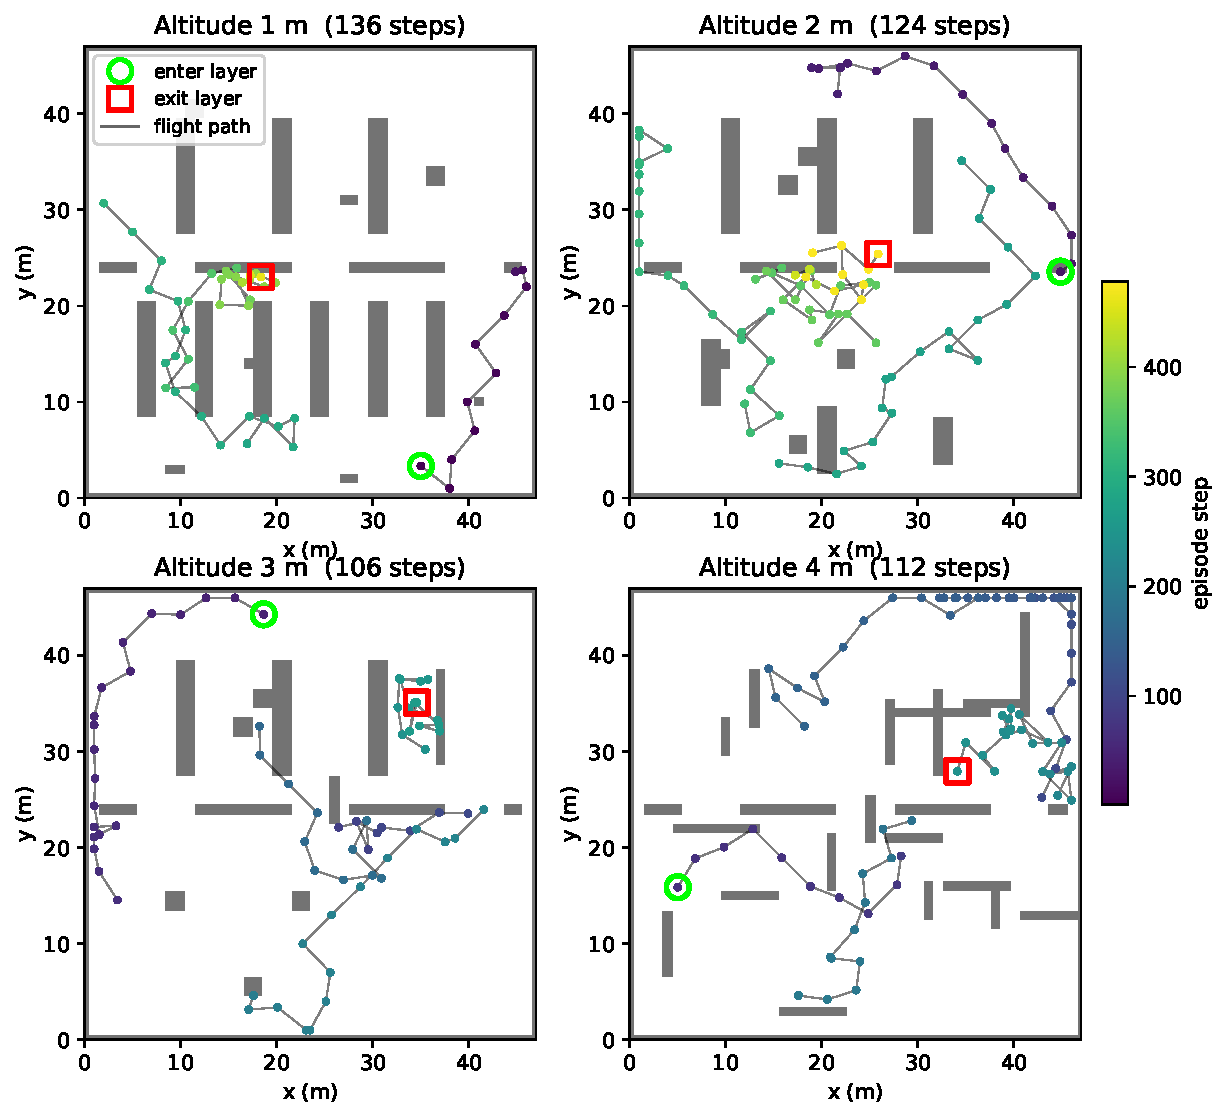
\includegraphics[width=0.82\textwidth]{figures/trajectory_altitudes_2x2.pdf}
\caption{A representative learned rollout on a held out map (one grid cell equals 1\,m). Each panel is one altitude layer, showing obstacles in grey and the agent path while flying at that height, coloured by episode step, with markers where the agent enters and leaves the layer. The policy spreads its effort evenly across all four layers rather than collapsing onto a single layer.}
\label{fig:traj}
\end{figure}

\section{Computational Cost and Sim-to-Real Transfer}

The policy is lightweight enough for onboard use. It has 2.02 million parameters and requires 10.16 million multiply accumulate operations per inference, and on a single CPU thread with no GPU it completes one inference in 1.20\,ms on average, which is far above the rate required for waypoint planning. The lightweight environment mirrors a Gazebo and PX4 stack in which RTAB-Map performs real time visual SLAM. Because the observation and action interfaces match the training environment, the trained policy runs in this stack without fine tuning and explores with stable odometry under an altitude cap. The dominant gap toward real hardware is motion smoothness, and we outline a roadmap that adds a motion smoothness reward, an altitude transition penalty, and a frontier definition aligned to the real mapping backend.

\section{Conclusion}

By making altitude an explicit decision and by shaping the reward around the localization signal, a single recurrent policy learns exploration that is more complete, balanced across altitudes, and faster, while remaining light enough to run on the vehicle. These results indicate that learned multi altitude active SLAM is a practical step toward UAVs that map unknown 3D spaces reliably on their own.

\end{document}
